\begin{figure*}[t]
\centering
\begin{tabular}{@{}c c c c c@{}} % @{} removes padding around the edge of the table
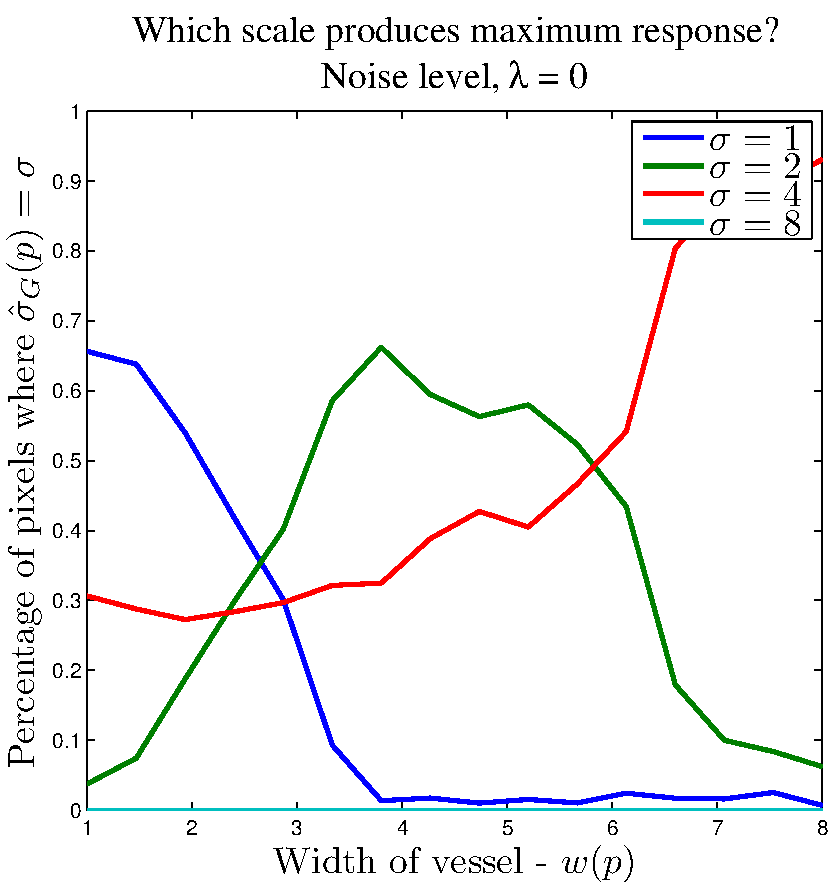
\includegraphics[width=0.18\textwidth]{figs/synthetic/syn_lines_g2d_scales_0} &
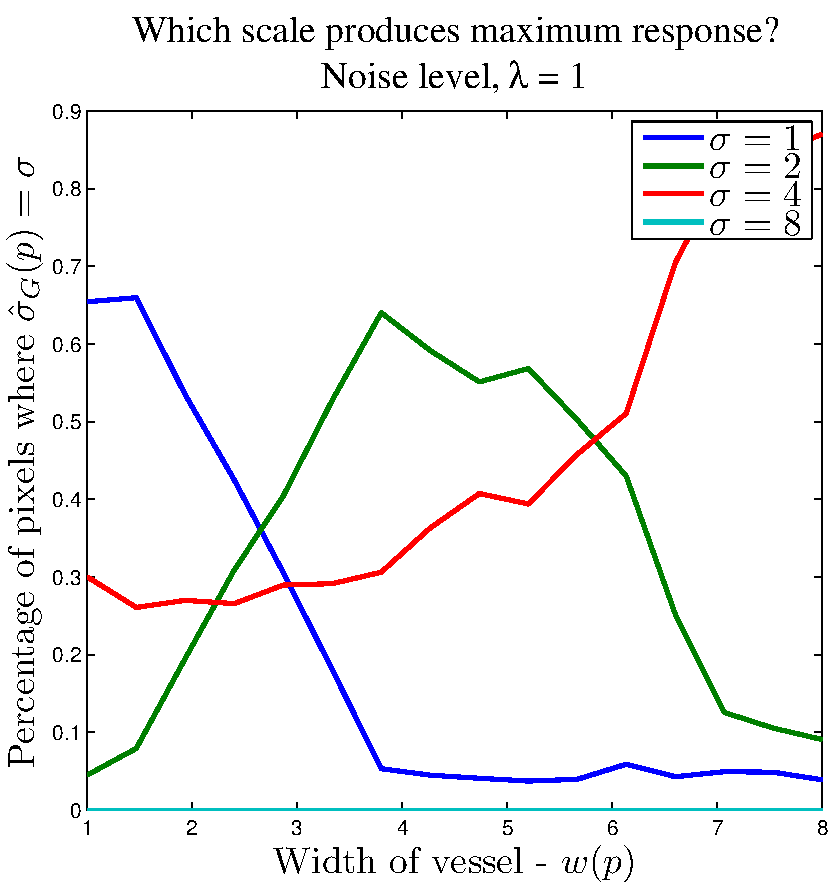
\includegraphics[width=0.18\textwidth]{figs/synthetic/syn_lines_g2d_scales_1} &
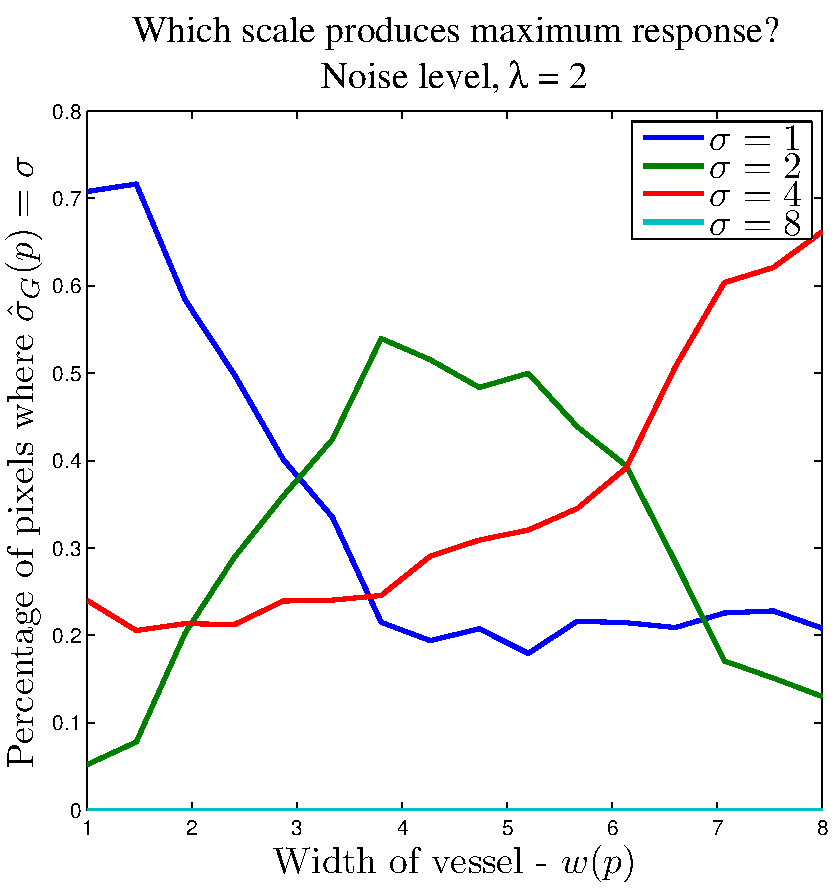
\includegraphics[width=0.18\textwidth]{figs/synthetic/syn_lines_g2d_scales_2} &
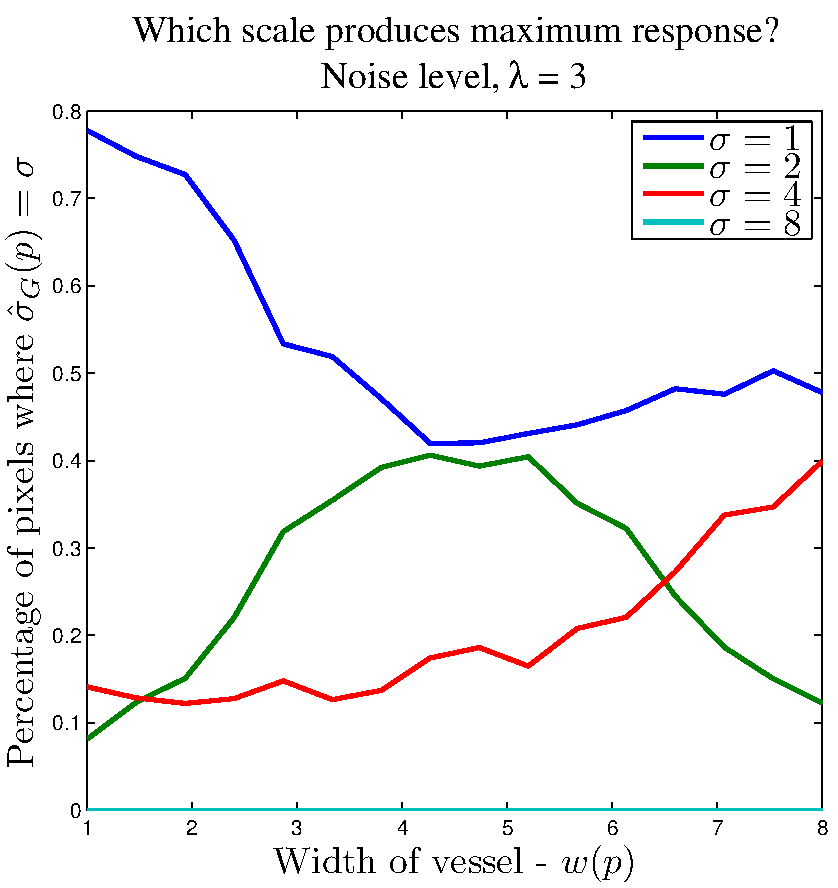
\includegraphics[width=0.18\textwidth]{figs/synthetic/syn_lines_g2d_scales_3} &
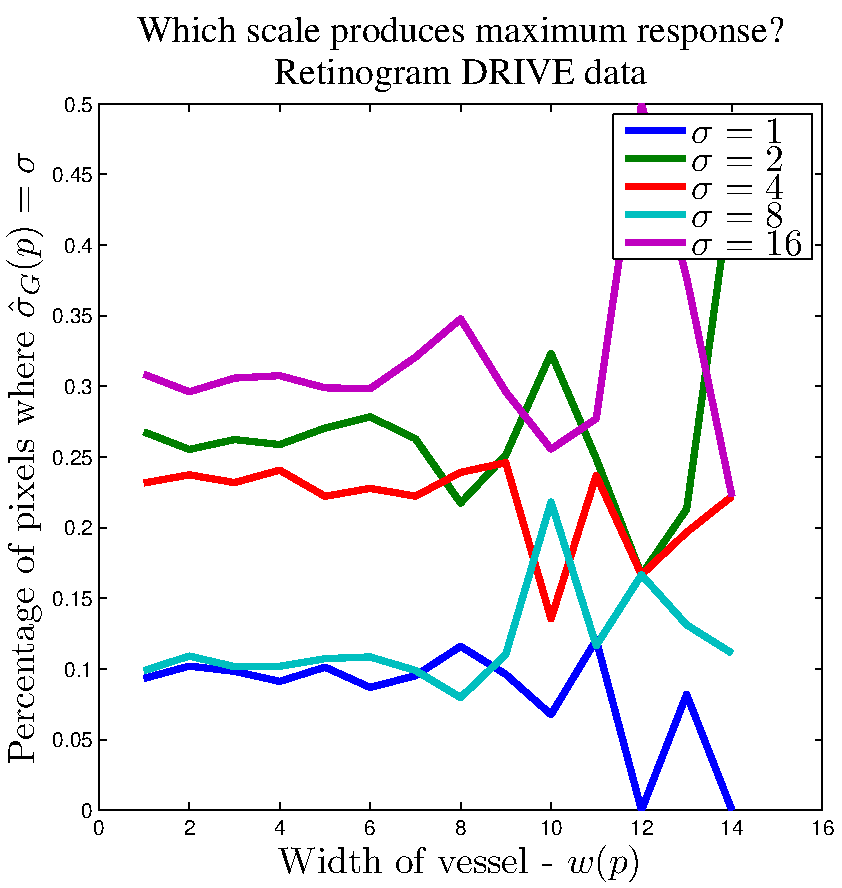
\includegraphics[width=0.18\textwidth]{figs/retina/ret_vessels_g2d_scales} \\
(a) & (b) & (c) & (d) & (e)\\
\noalign{\smallskip}

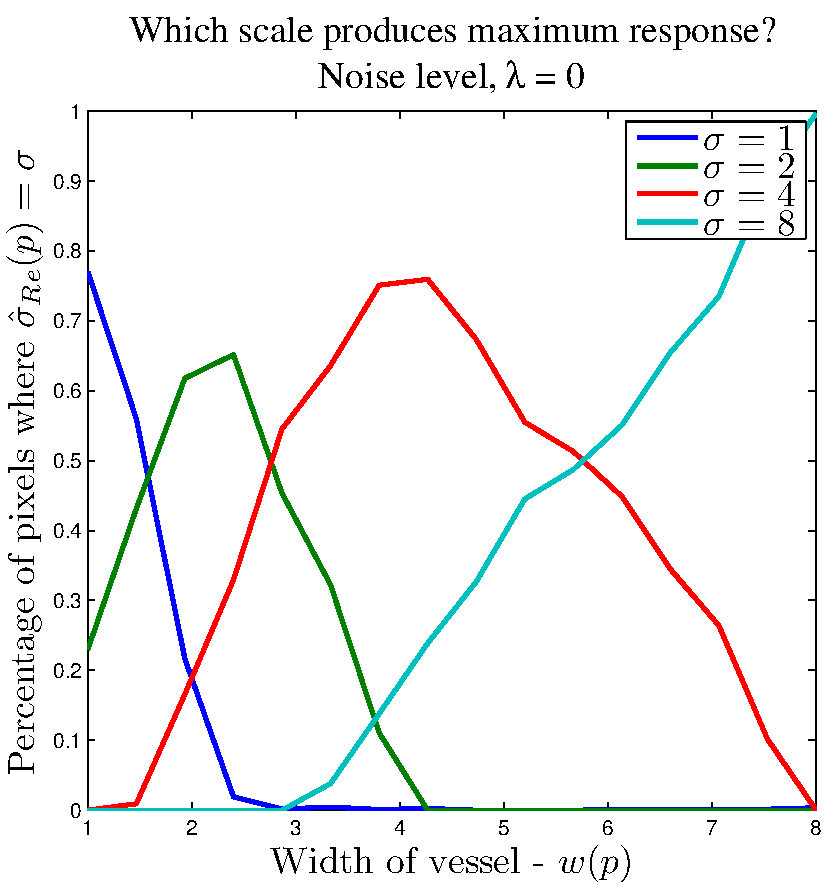
\includegraphics[width=0.18\textwidth]{figs/synthetic/syn_lines_gabor_scales_0} &
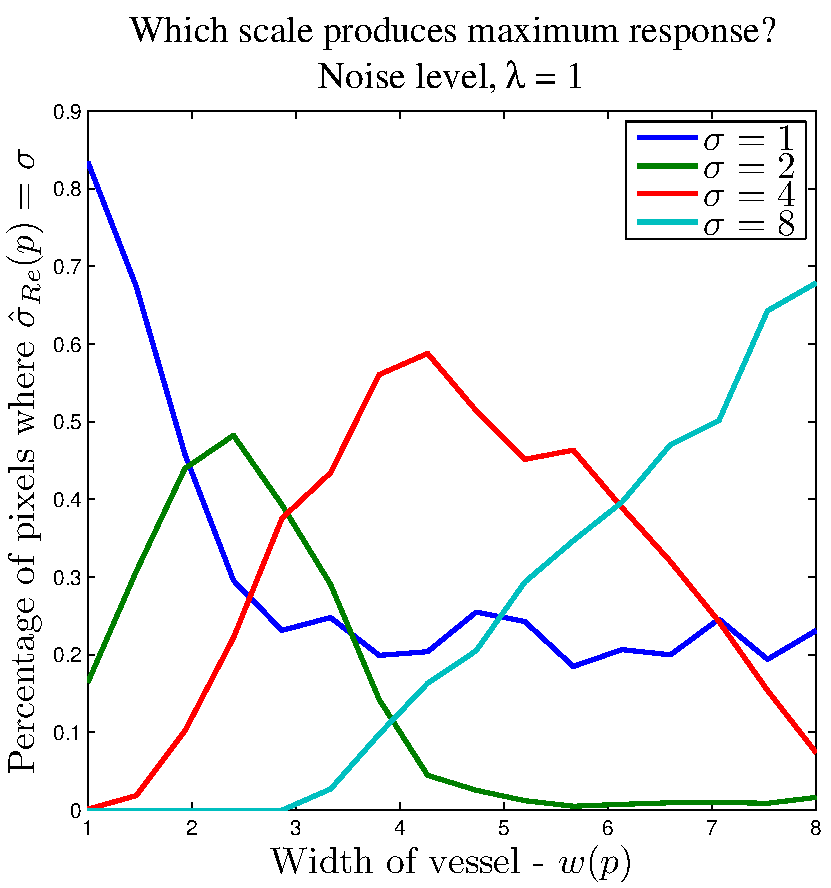
\includegraphics[width=0.18\textwidth]{figs/synthetic/syn_lines_gabor_scales_1} &
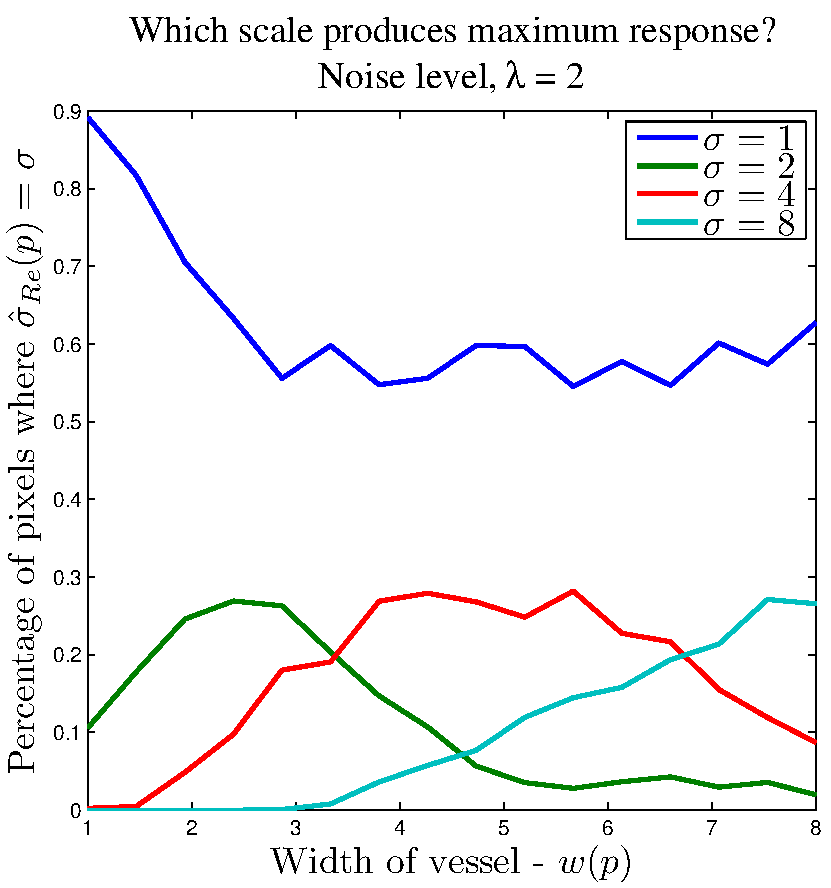
\includegraphics[width=0.18\textwidth]{figs/synthetic/syn_lines_gabor_scales_2} &
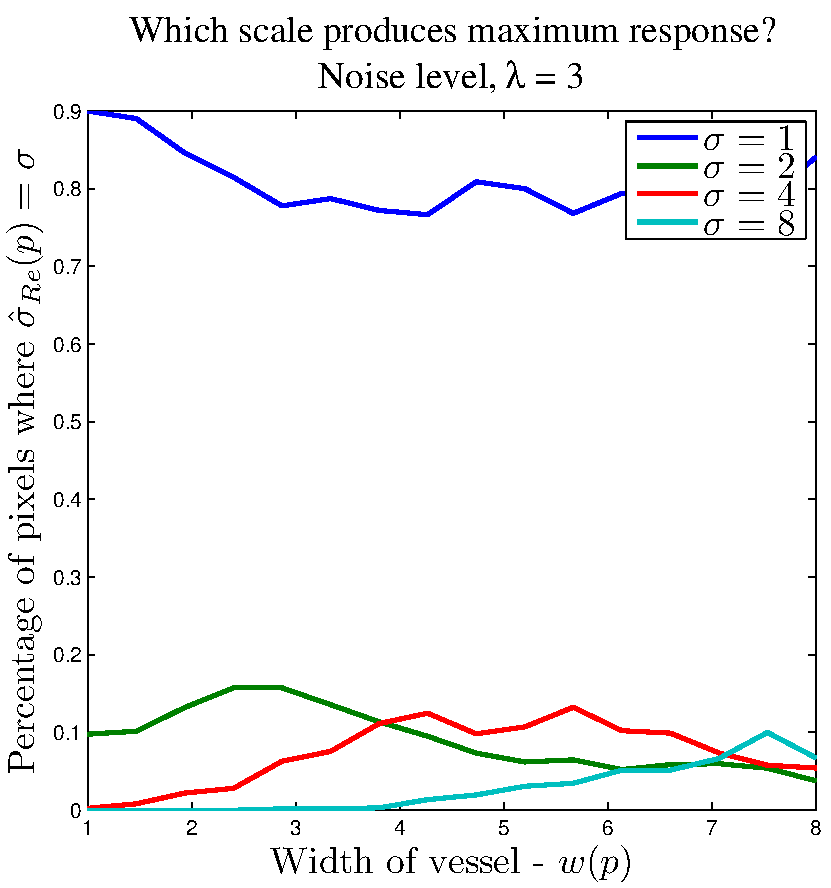
\includegraphics[width=0.18\textwidth]{figs/synthetic/syn_lines_gabor_scales_3} &
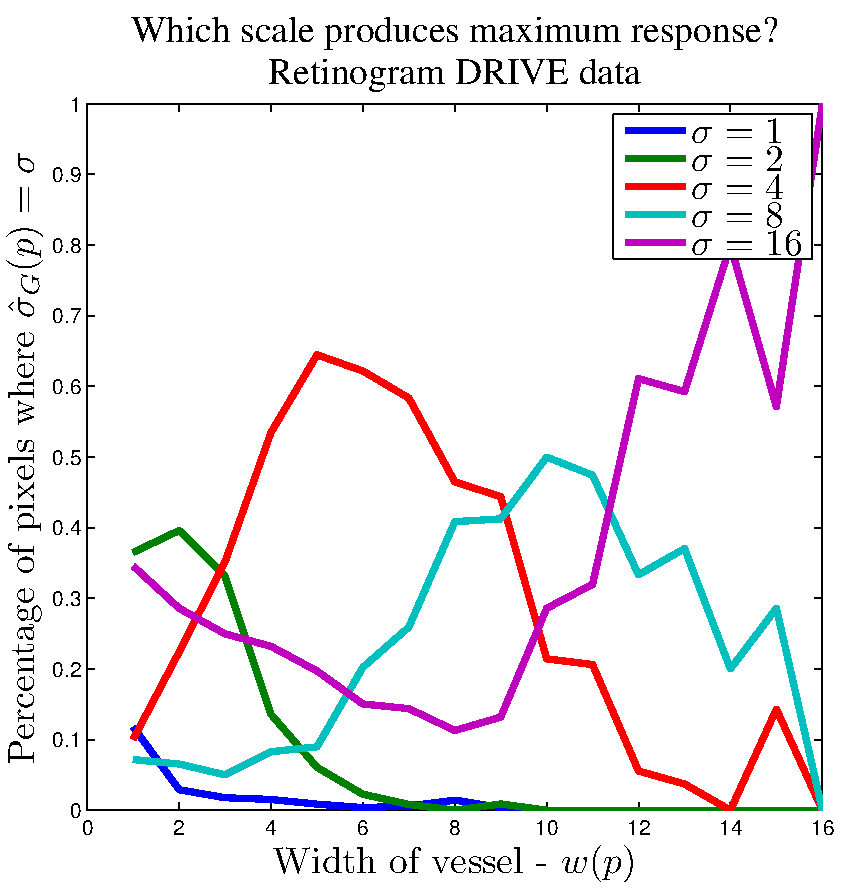
\includegraphics[width=0.18\textwidth]{figs/retina/ret_vessels_gabor_scales} \\
(f) & (g) & (h) & (i) & (j)\\
\noalign{\smallskip}

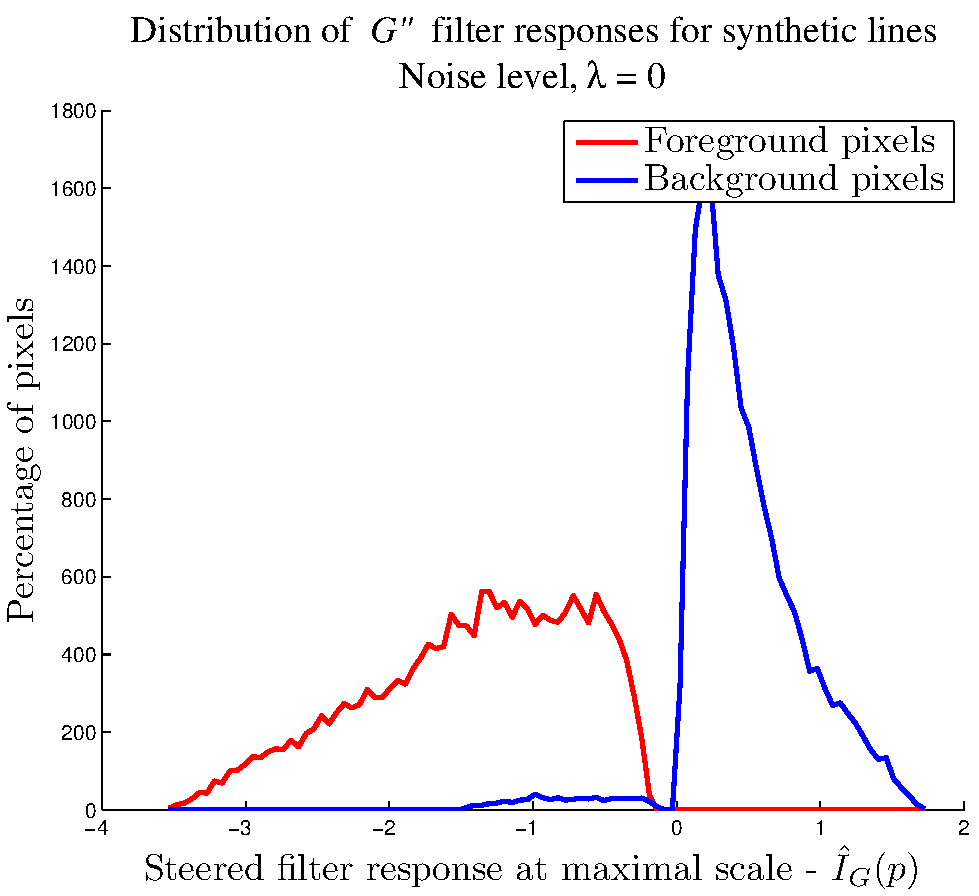
\includegraphics[width=0.18\textwidth]{figs/synthetic/syn_lines_g2d_responses_cdf_0} &
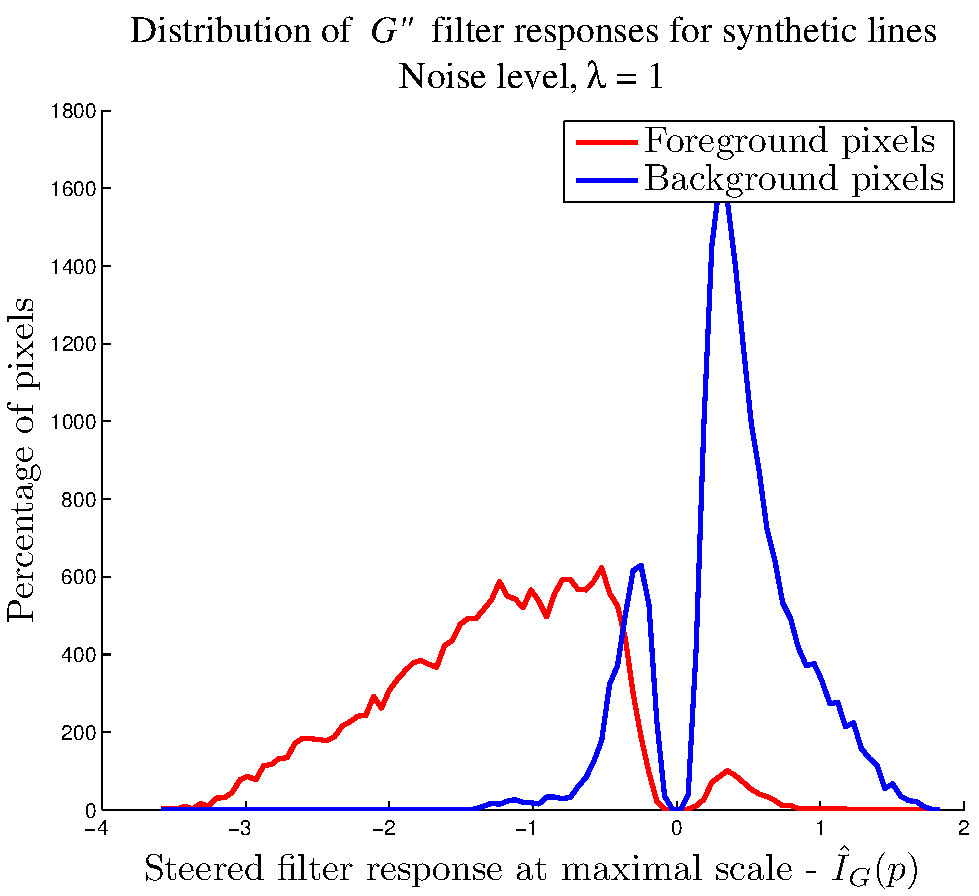
\includegraphics[width=0.18\textwidth]{figs/synthetic/syn_lines_g2d_responses_cdf_1} &
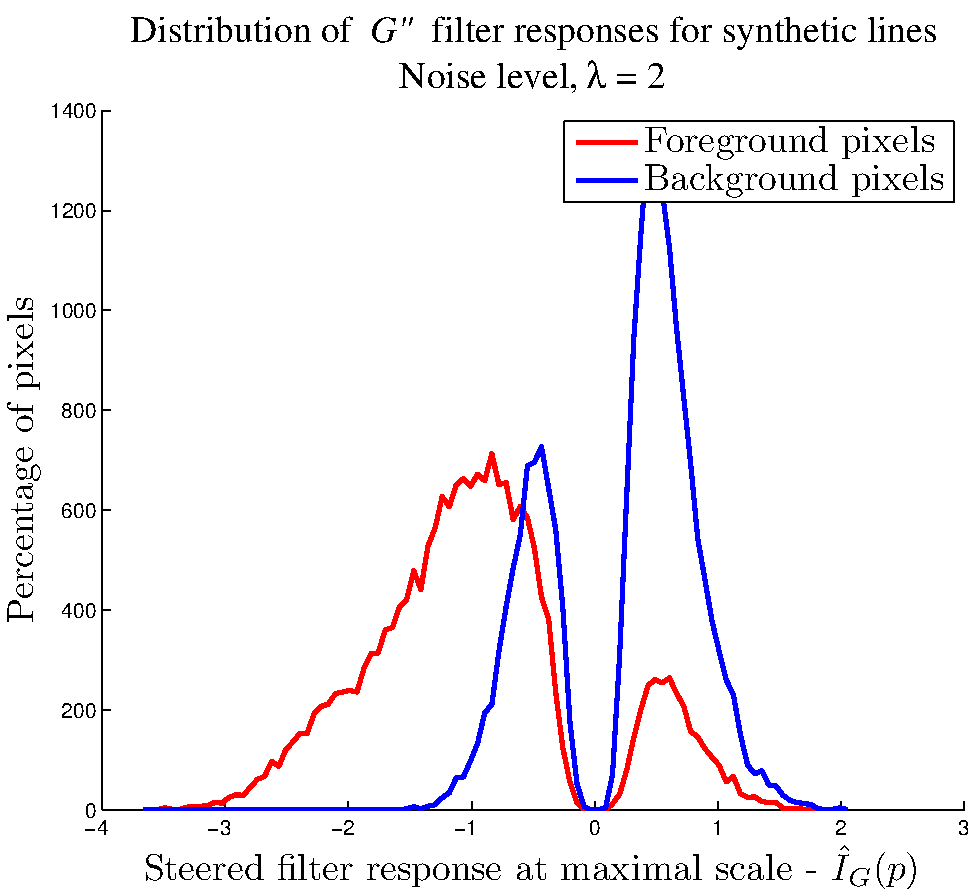
\includegraphics[width=0.18\textwidth]{figs/synthetic/syn_lines_g2d_responses_cdf_2} &
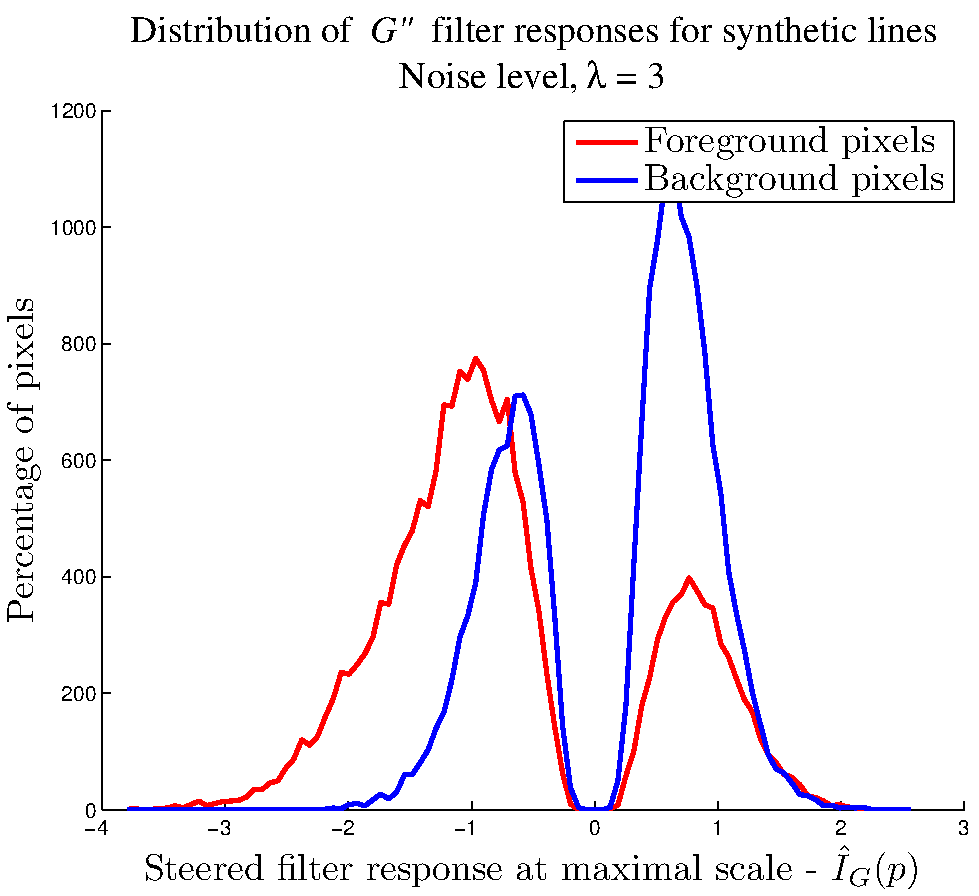
\includegraphics[width=0.18\textwidth]{figs/synthetic/syn_lines_g2d_responses_cdf_3} &
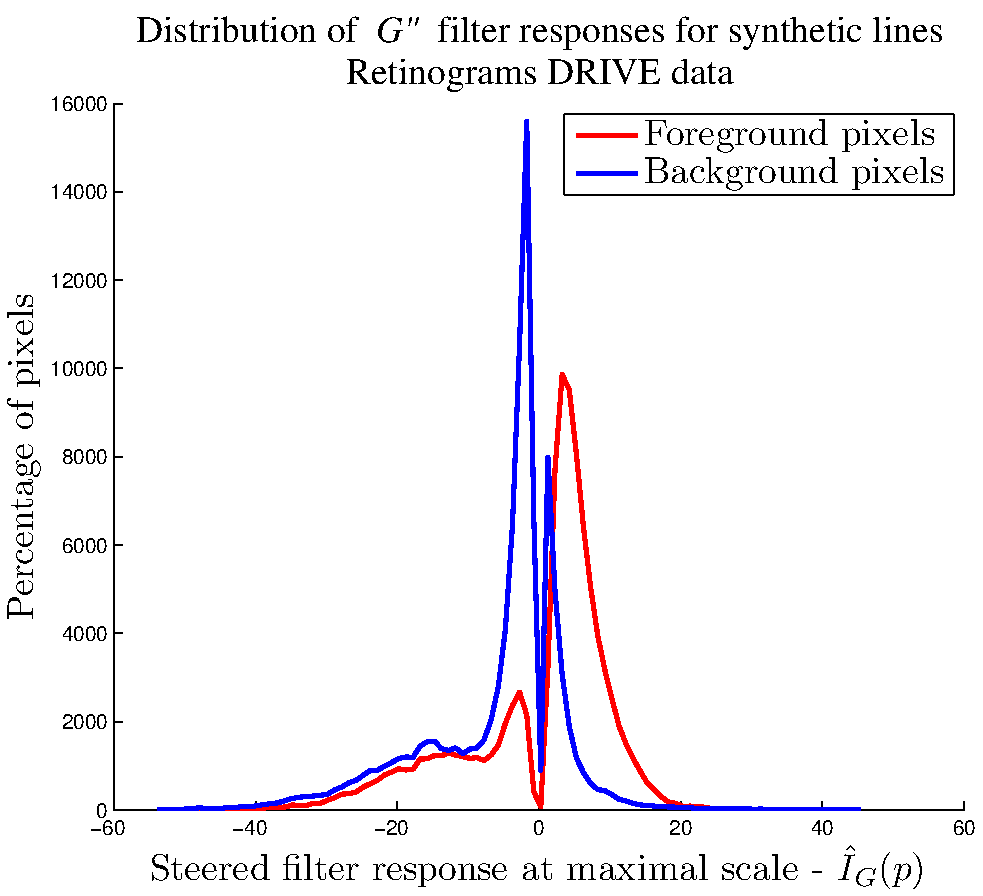
\includegraphics[width=0.18\textwidth]{figs/retina/ret_vessels_g2d_responses_cdf}  \\
(k) & (l) & (m) & (n) & (o)\\
\noalign{\smallskip}

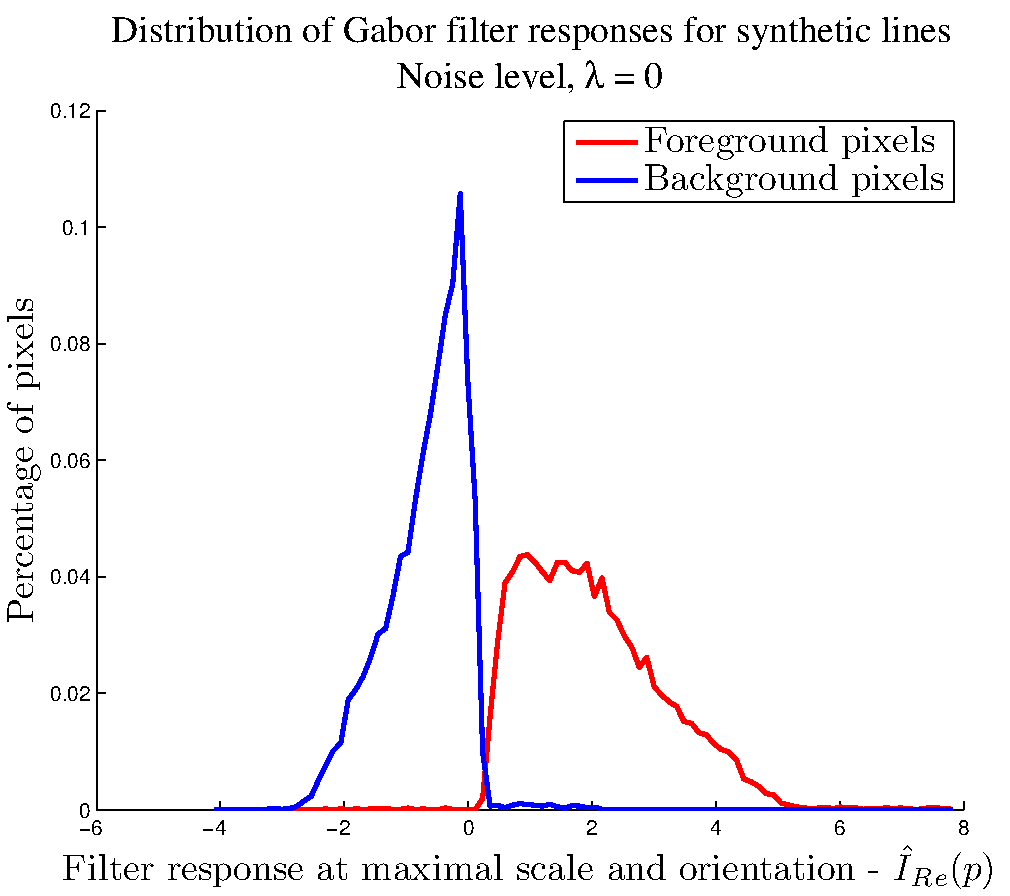
\includegraphics[width=0.18\textwidth]{figs/synthetic/syn_lines_gabor_responses_cdf_0} &
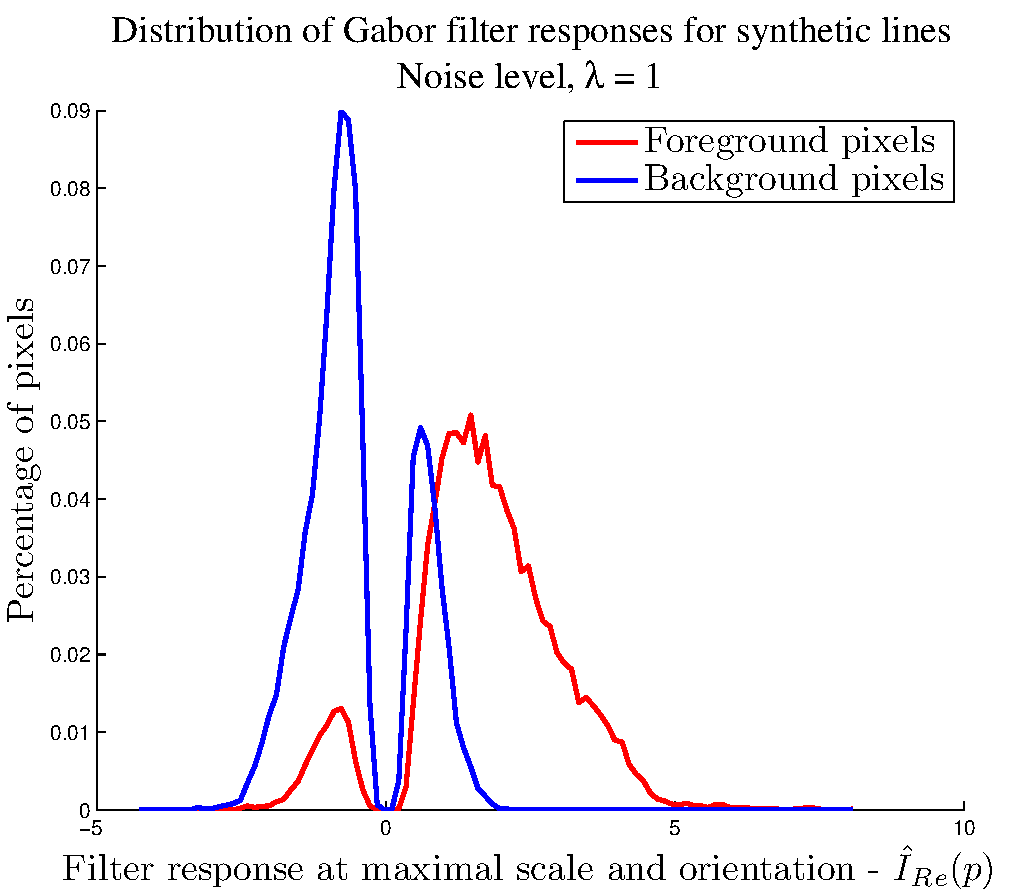
\includegraphics[width=0.18\textwidth]{figs/synthetic/syn_lines_gabor_responses_cdf_1} &
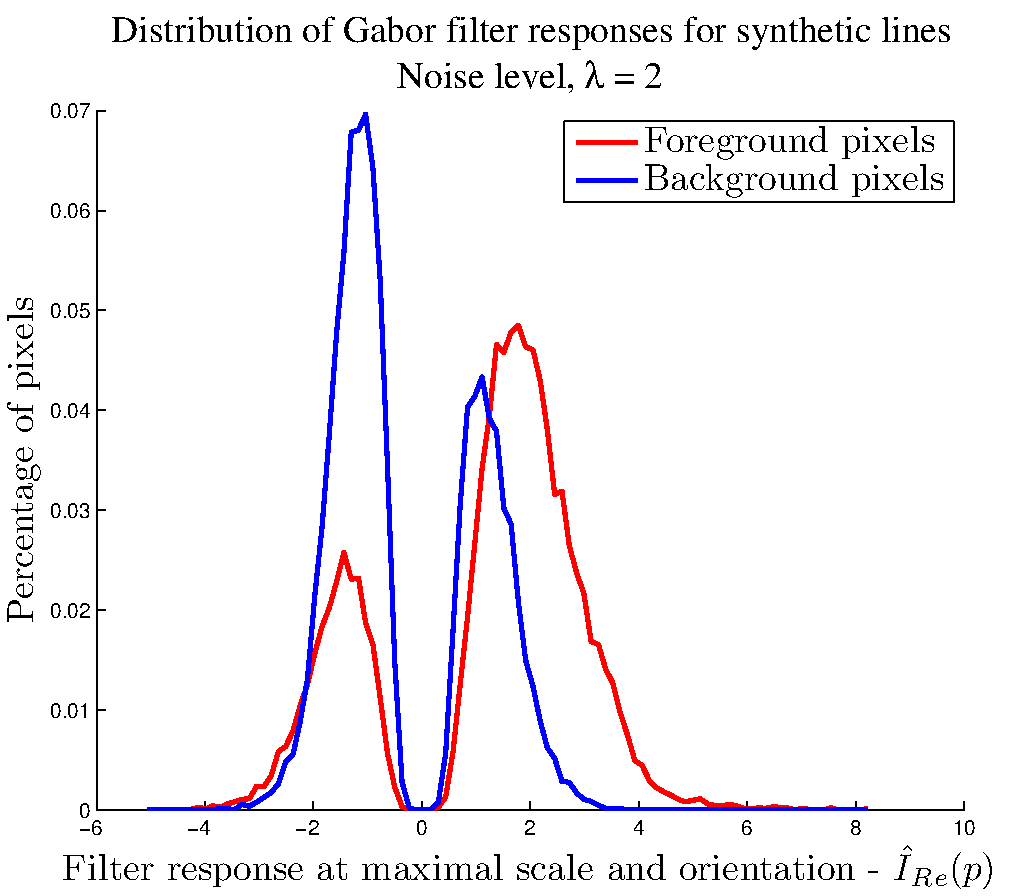
\includegraphics[width=0.18\textwidth]{figs/synthetic/syn_lines_gabor_responses_cdf_2} &
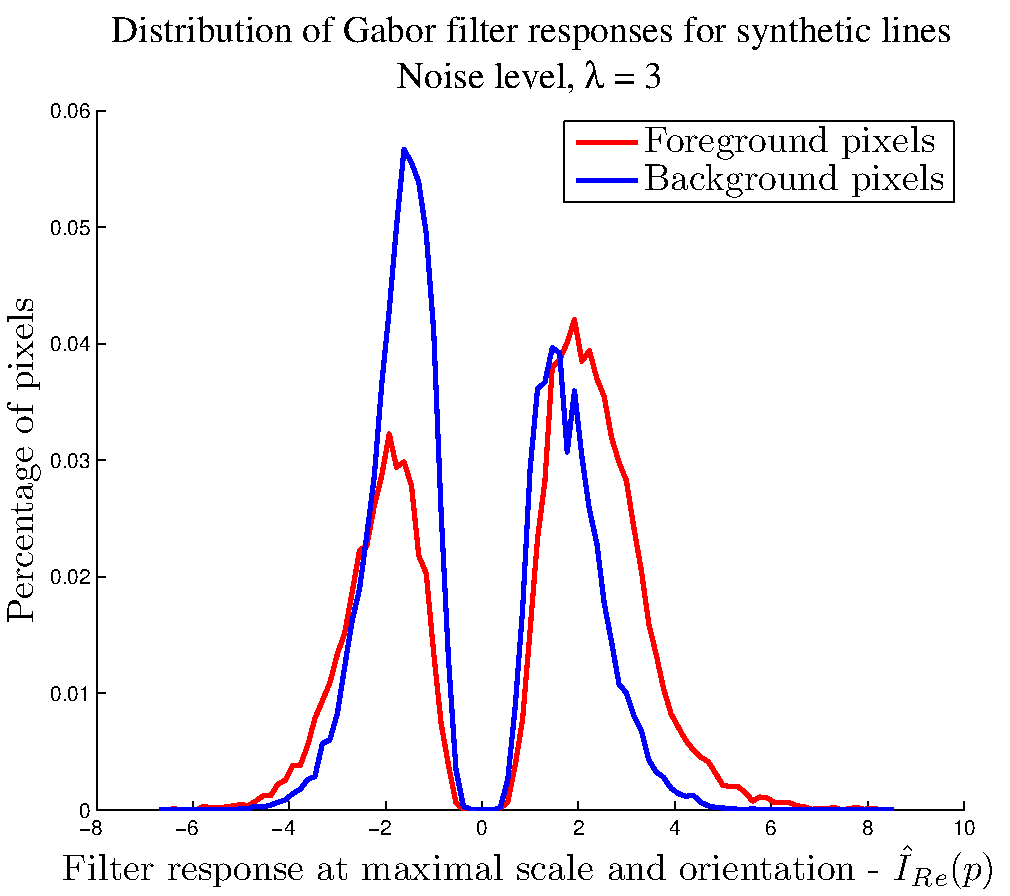
\includegraphics[width=0.18\textwidth]{figs/synthetic/syn_lines_gabor_responses_cdf_3} &
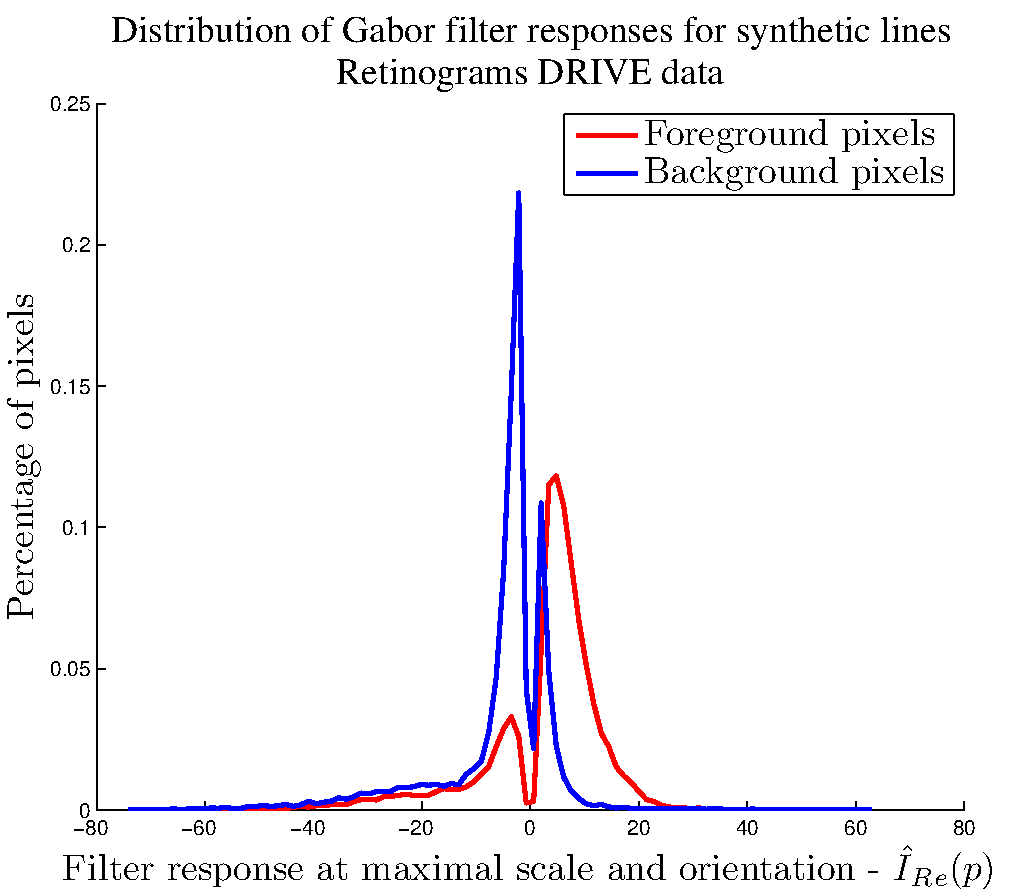
\includegraphics[width=0.18\textwidth]{figs/retina/ret_vessels_gabor_responses_cdf} \\
(p) & (q) & (r) & (s) & (t)\\
\noalign{\smallskip}

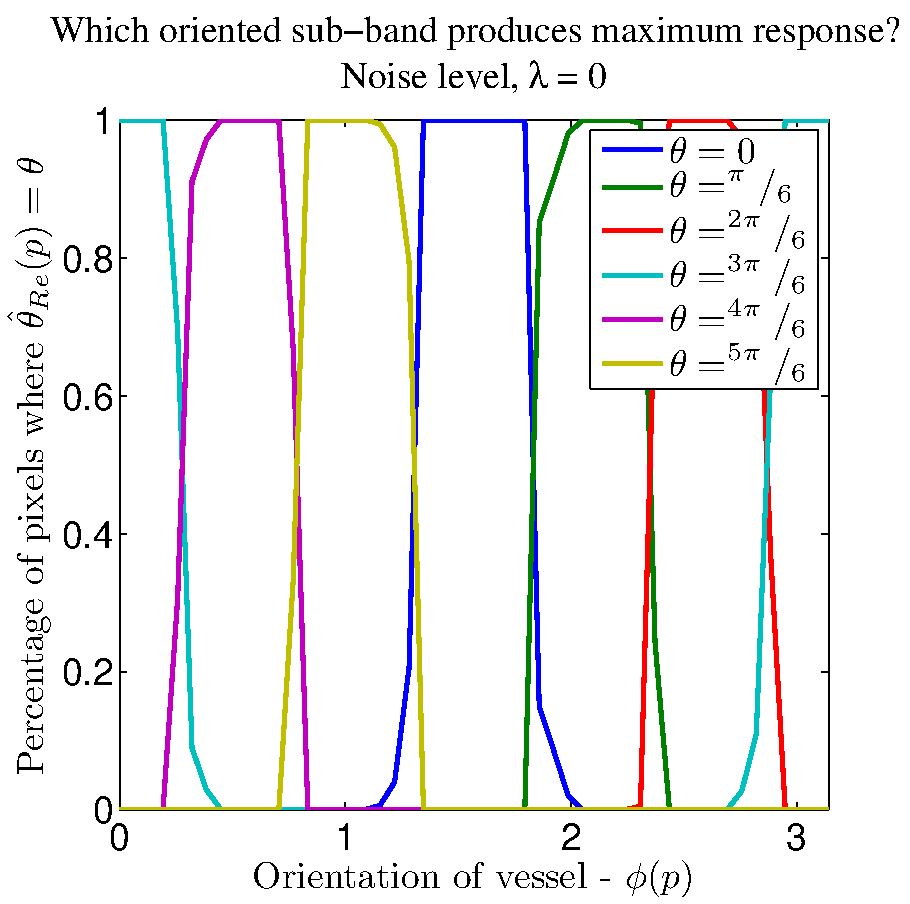
\includegraphics[width=0.18\textwidth]{figs/synthetic/syn_lines_gabor_ori_subbands_0} &
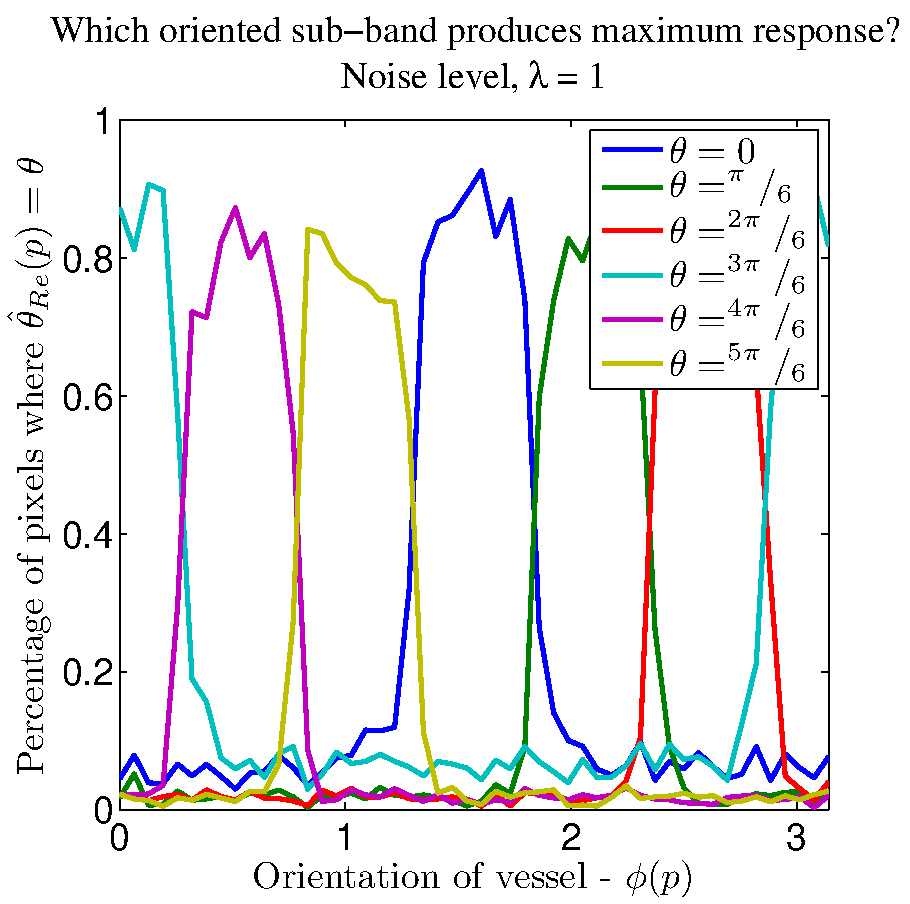
\includegraphics[width=0.18\textwidth]{figs/synthetic/syn_lines_gabor_ori_subbands_1} &
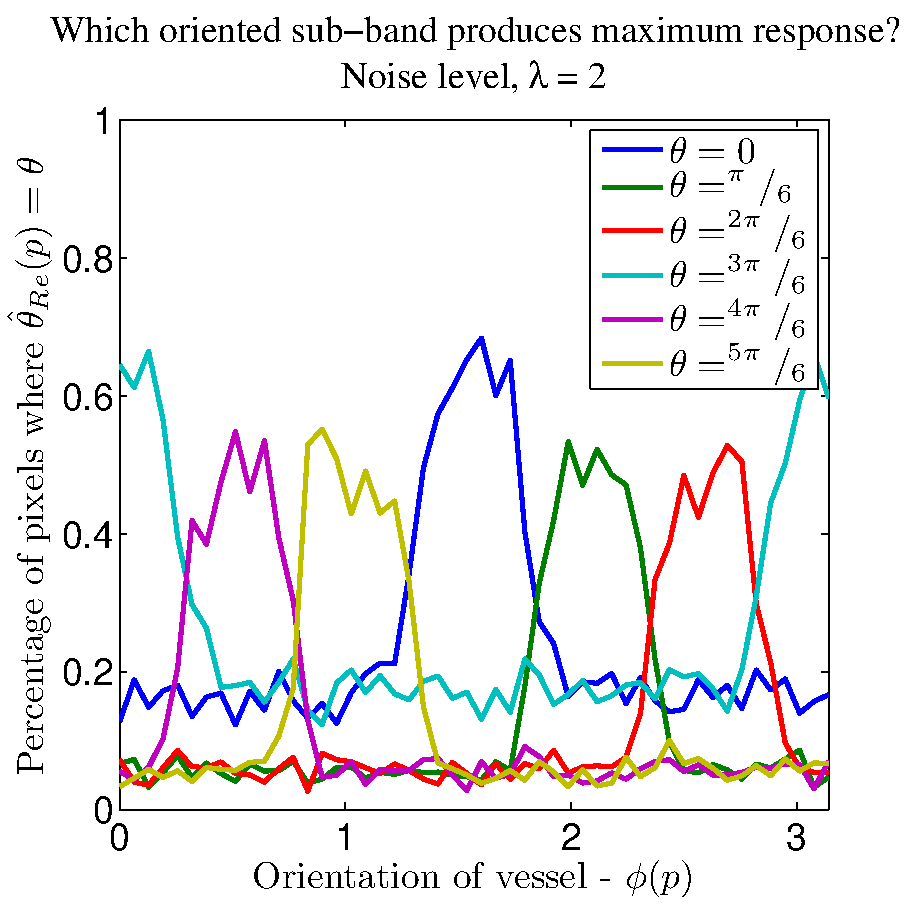
\includegraphics[width=0.18\textwidth]{figs/synthetic/syn_lines_gabor_ori_subbands_2} &
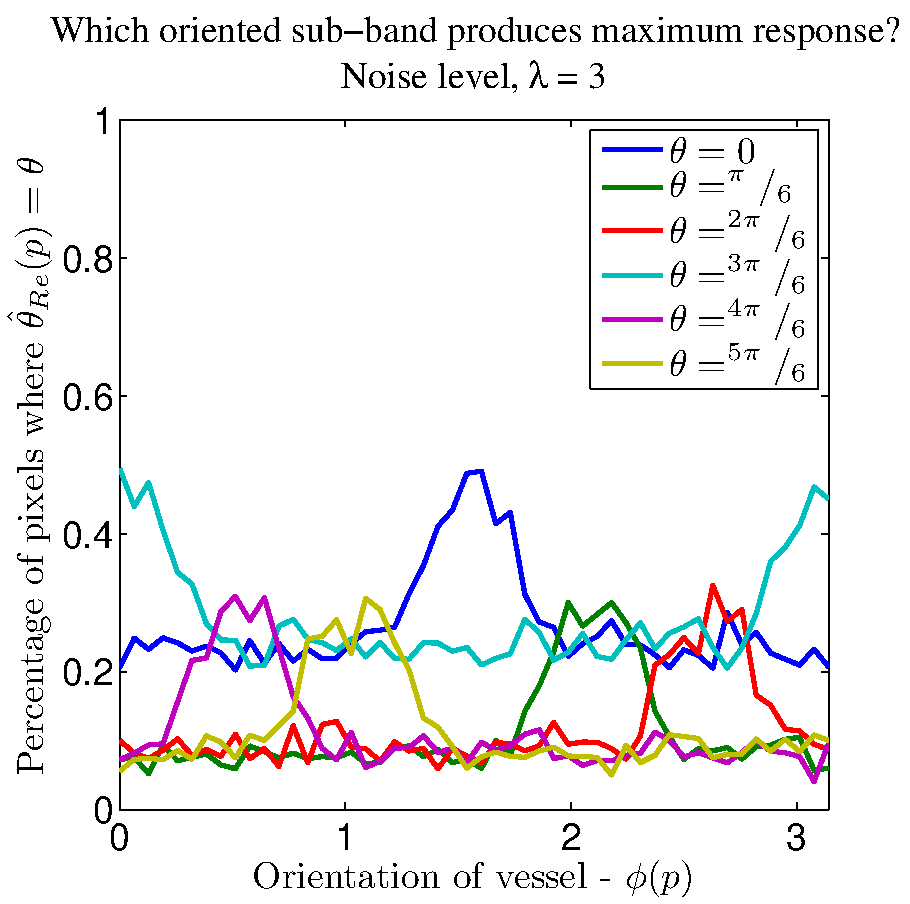
\includegraphics[width=0.18\textwidth]{figs/synthetic/syn_lines_gabor_ori_subbands_3} &
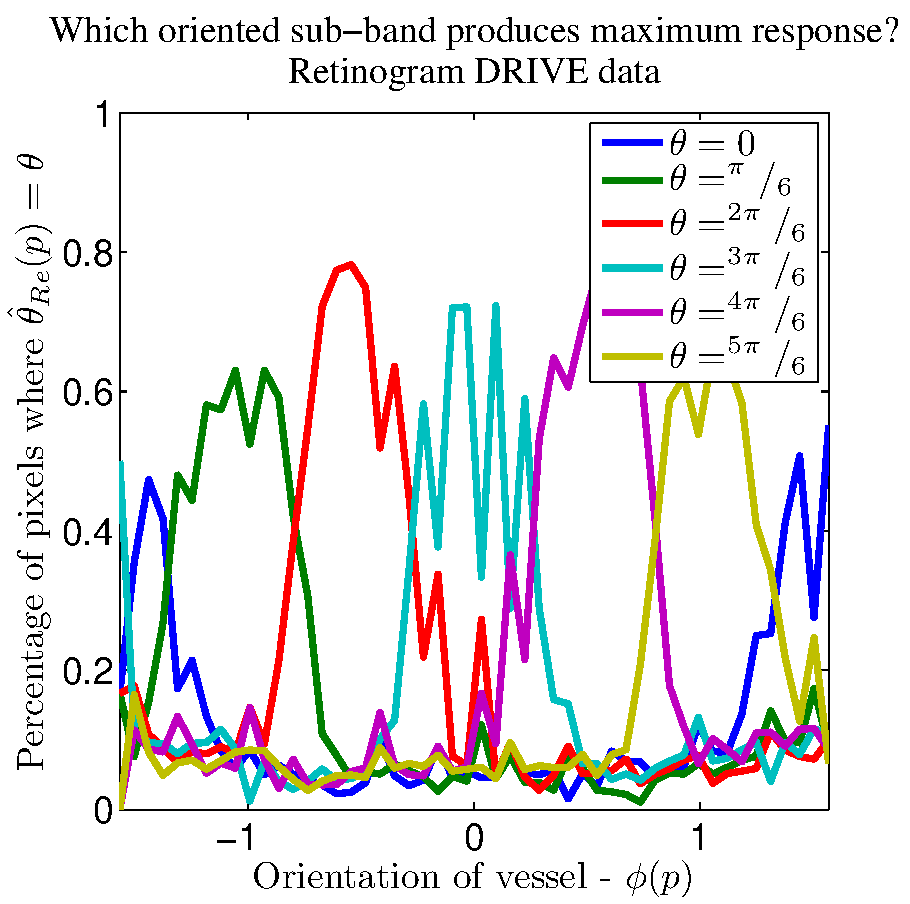
\includegraphics[width=0.18\textwidth]{figs/retina/ret_vessels_gabor_ori_subbands} \\
(u) & (v) & (w) & (x) & (y)\\
\noalign{\smallskip}

\end{tabular}
%
\caption{\emph{Columns from left to right} show results for different datasets: (a-d) synthetic images with noise level of $\eta$ set to 0, 1, 2 and 3 respectively; (e) DRIVE retinograms. Rows top to bottom show: Scale response as a function of CLS width to Gaussian filters(a-e) and Gabor filters (f-j); CLS and background response distribution for Gaussian filters (k-o) and Gabor filters (p-t); Gabor filter response as a function of CLS orientation (u-y).}
\label{f:synthetic_exp1}
\end{figure*}
